\documentclass[10pt,a4paper]{article}
\usepackage[utf8]{inputenc}
\usepackage{amsfonts}
\usepackage{graphicx}
\graphicspath{ {images/} }
\usepackage{indentfirst}
\usepackage{float}
\usepackage{listings}

\lstset{
  basicstyle=\ttfamily,
  columns=fullflexible,
  frame=single,
  breaklines=true,
}

\begin{document}

\title{EncryptZip: \\ Compressed, Encrypted Containers on Android \\ Project Milestone}
\author{Alex Shah}
\date{4/7/18}

\maketitle

\section{Abstract}
This project sets out to implement encryption on zip based containers on the Android platform. This was accomplished with tools available in the Android SDK Java. Containers are created by zipping a folder's contents on the user's device. Zipping a folder compresses it to save file size. A key is generated using SHA-256 from the user's provided password. The zip container is then encrypted with AES using the generated key. These containers are thereby compressed, encrypted, and inherently portable.

\section{Introduction}
Encrypting files is a common practice to prevent unauthorized or unintended access to sensitive information. However, encrypting each file is only one facet of security in a system. Encrypting the container which sensitive information is held can prove more useful than encrypting on a per file basis, or in addition to it. This is especially useful in applications where the system cannot be entirely secured. It can be used in addition to measures such as file and disk based encryption schemes. These three levels, file level, container level, and system/disk level encryption ensure that access is compartmentalized and can further secure a user's documents from unwanted access. 

\section{Background}
While desktop operating systems have applications to create encrypted containers, such as Veracrypt, Android does not have a native application and third party implementations use proprietary methods. In addition, solutions such as Veracrypt create fixed sized containers regardless of the size of the contents of the container. This is especially important in the mobile environment where space is at a premium and transmission of containers over a network may prove limited. The goal of this project is to use built in features and standard systems to create a container level encryption scheme on the Android mobile platform which solves these problems by using compressed zip archives.

\section{Methodology}
Utilizing the Android SDK and available cryptography libraries provided by Google and within Java, it is feasible to zip and encrypt the files on the emulated storage on an Android device. Using java.io and java.zip libraries, the users documents are compressed in a zip archive. A key is generated using SHA-256 with a provided password. This key is then used with AES from the javax.crypto library to encrypt the byte stream of the zip contents. The resulting file is unreadable but using the reverse procedure can be recovered fully. The encrypted zip is not affected by incorrect decryption, using the methods implemented. The encryption must use a password, as no password would be insecure, or at worst a randomly generated key would not be able to be decrypted. Users can also use built in Google drive support to store, share, or keep an encrypted zip container synchronized between devices.

\section{Experiments}
To implement directory zipping in Android it is necessary to use a buffer and an InputStream. For example:

\begin{lstlisting}[language=Java]
fileOutputStream = new FileOutputStream(file);
zipOutputStream = new ZipOutputStream(new BufferedOutputStream(fileOutputStream));

byte data[] = new byte[BUFFER_SIZE];
FileInputStream fileInputStream = new FileInputStream(file.getPath());
input = new BufferedInputStream(fileInputStream, BUFFER_SIZE);
entryPath = file.getAbsolutePath().replace(parentPath, "");
ZipEntry entry = new ZipEntry(entryPath);
zipOutputStream.putNextEntry(entry);
int count;
while ((count = input.read(data, 0, BUFFER_SIZE)) != -1) {
  zipOutputStream.write(data, 0, count);
}
input.close();

\end{lstlisting}

It is necessary to use some additional libraries. These include security and extension libraries separate from the base Java libraries. These include:

\begin{lstlisting}[language=Java]
import java.security.NoSuchAlgorithmException;
import java.security.spec.InvalidKeySpecException;
import java.security.spec.KeySpec;
import javax.crypto.Cipher;
import javax.crypto.spec.PBEKeySpec;
\end{lstlisting}

These enable us to securely generate a 256 bit key using the provided password as well as encrypt the zip using AES with a 256 bit key, better than the 128 bits required and greater key length than what our in class implementation allowed.

In order to encrypt the zip, javax crypto and java security libraries are used in accordance to Android's security guidelines to perform SHA 256 and AES using a 256 bit key.
\begin{lstlisting}[language=Java]
// generate key from password using AES
    public static SecretKey generateKey(char[] password) throws NoSuchAlgorithmException, InvalidKeySpecException {
        final int iterations = 1000;

        // Generate a 256-bit key with SHA256
        final int outputKeyLength = 256;
        byte[] salt = new byte[20];

        SecretKeyFactory secretKeyFactory = SecretKeyFactory.getInstance("PBKDF2withHmacSHA256");
        KeySpec keySpec = new PBEKeySpec(password, salt, iterations, outputKeyLength);
        SecretKey secretKey = secretKeyFactory.generateSecret(keySpec);
        return secretKey;
    }

    // encrypt with AES
    public static byte[] encrypt(SecretKey key, byte[] fileData) throws Exception {
        Cipher cipher = Cipher.getInstance("AES");
        cipher.init(Cipher.ENCRYPT_MODE, key);
        byte[] encrypted = cipher.doFinal(fileData);
        return encrypted;
    }

\end{lstlisting}

\clearpage

\section{App}

The main screen of the EncryptZip app. The zip, unzip, encrypt, and decrypt buttons function as anticipated, and in that order to create a container and to open it.
\begin{figure}[H]
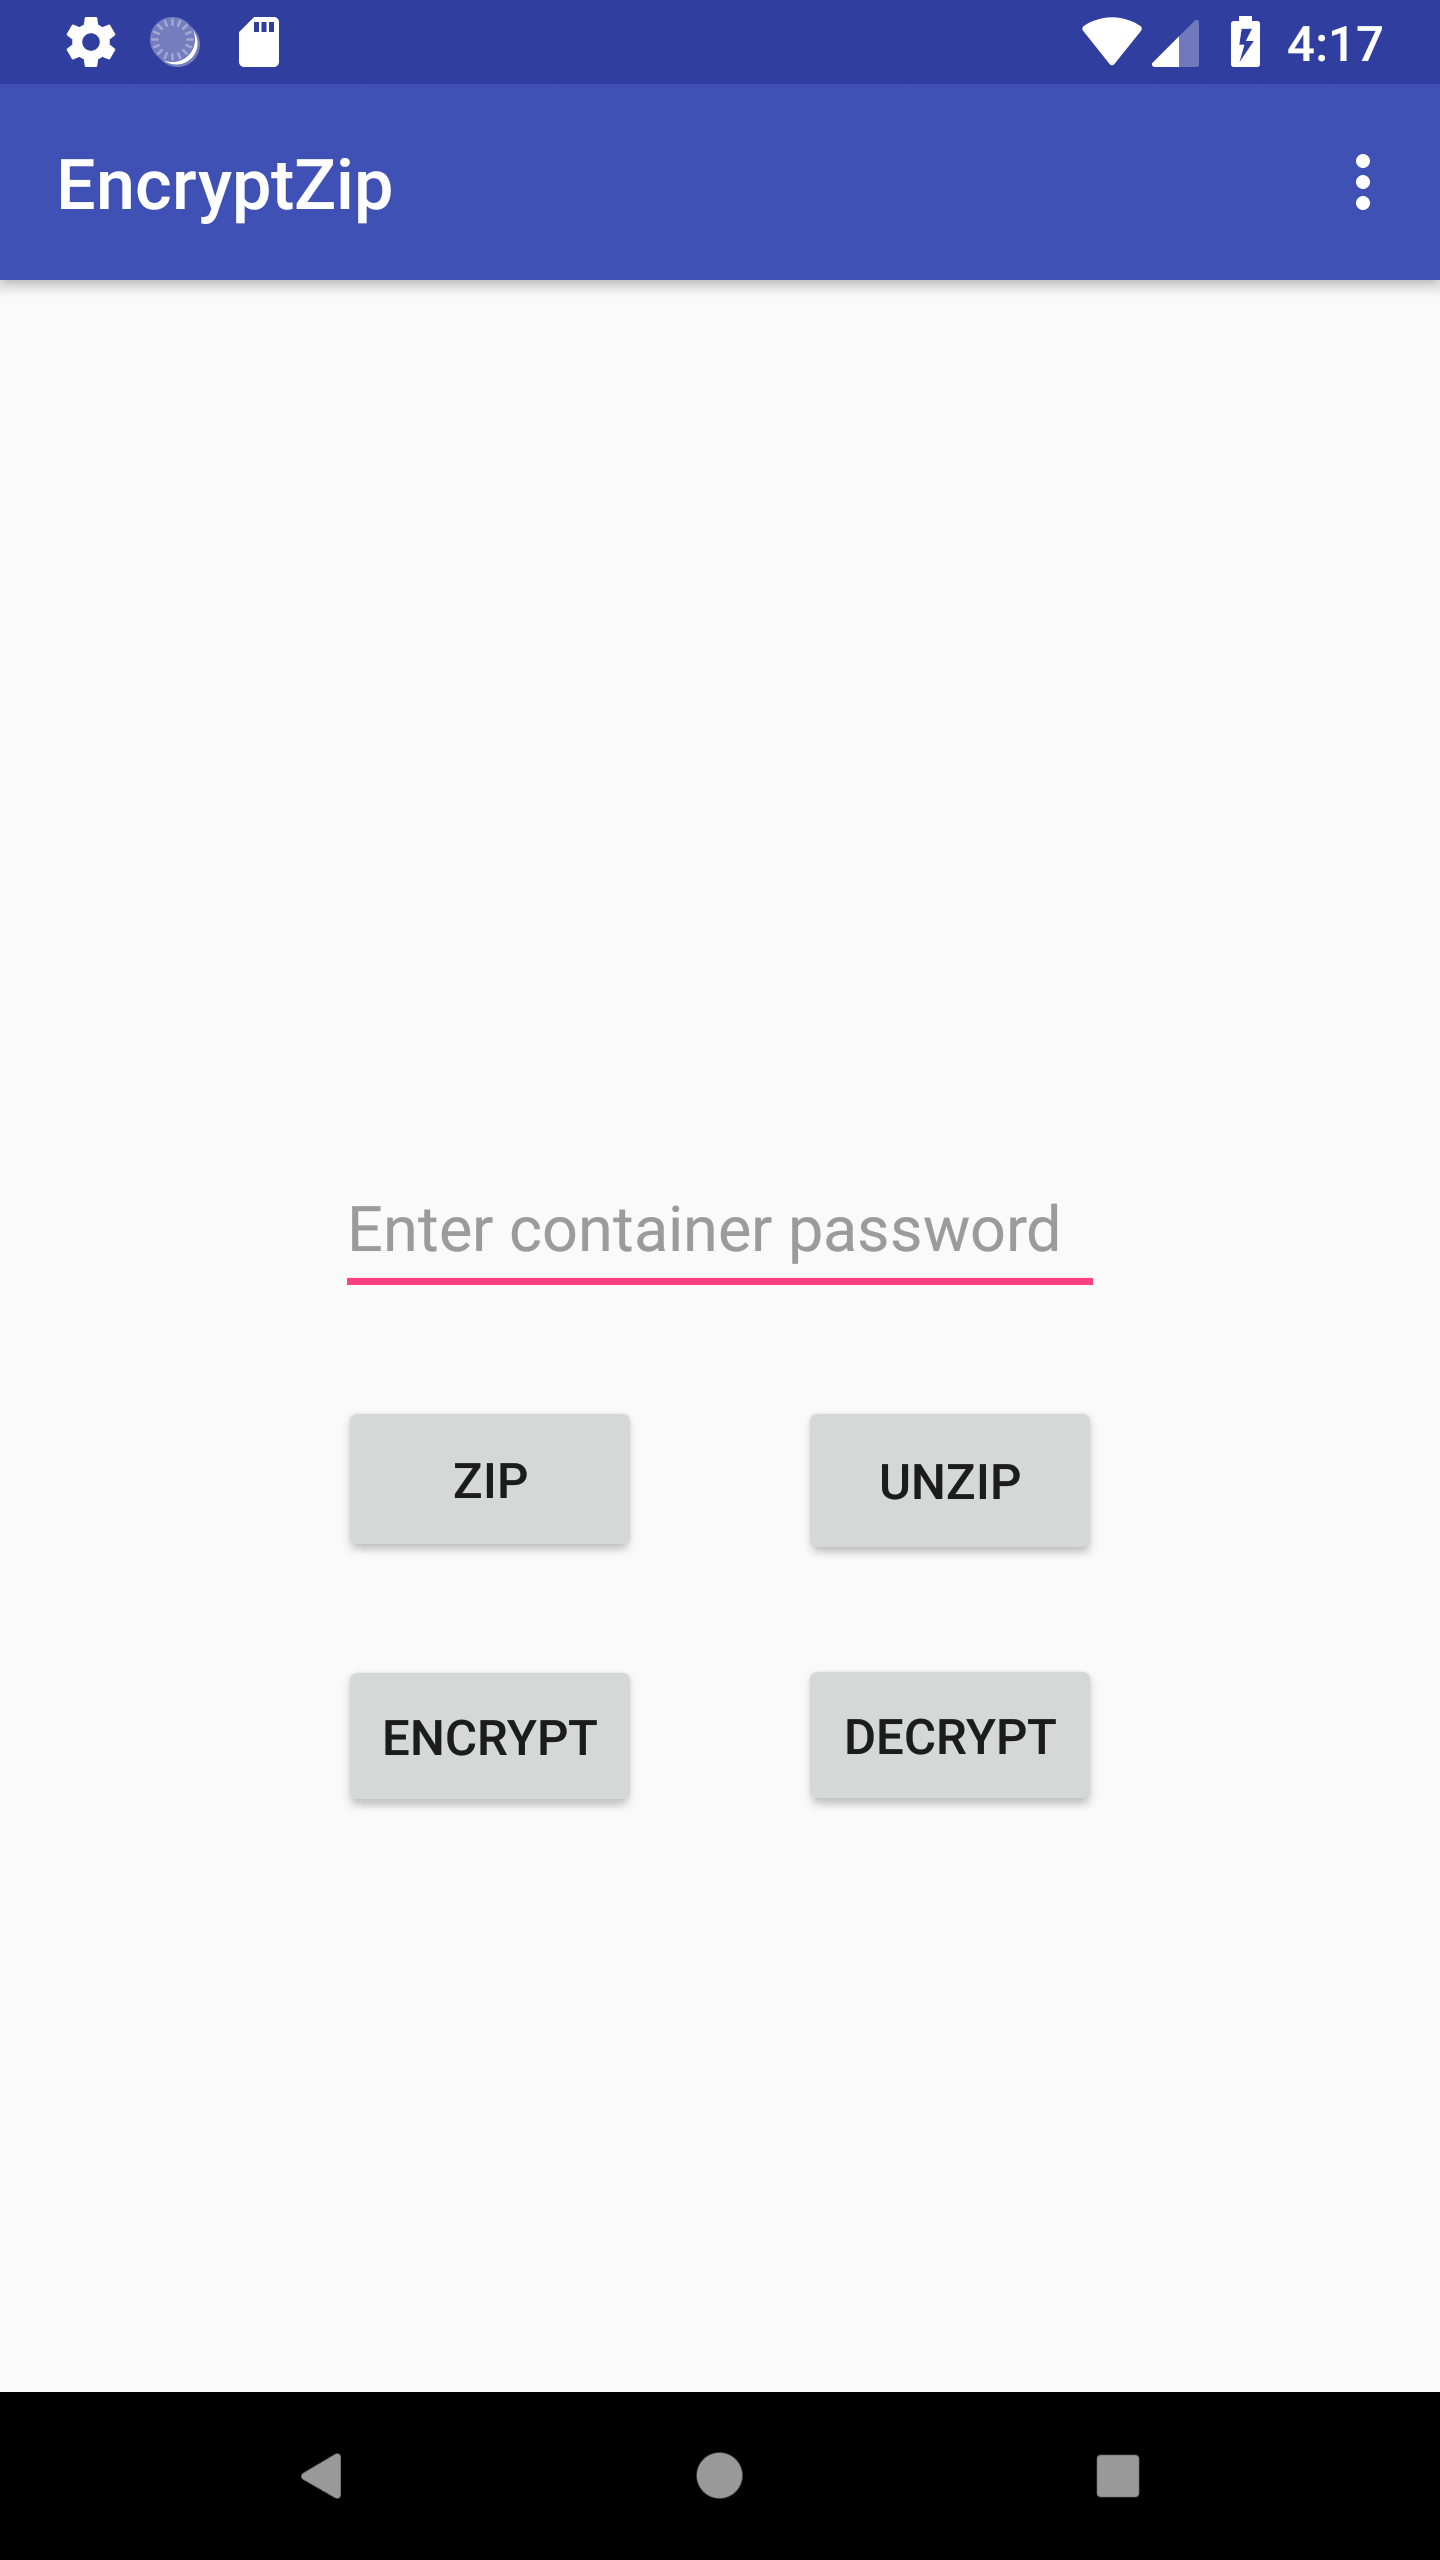
\includegraphics[width=8cm]{main1}
\end{figure}

\clearpage

Toast notifications are shown to the user to indicate whether an action has completed successfully or not.
\begin{figure}[h]
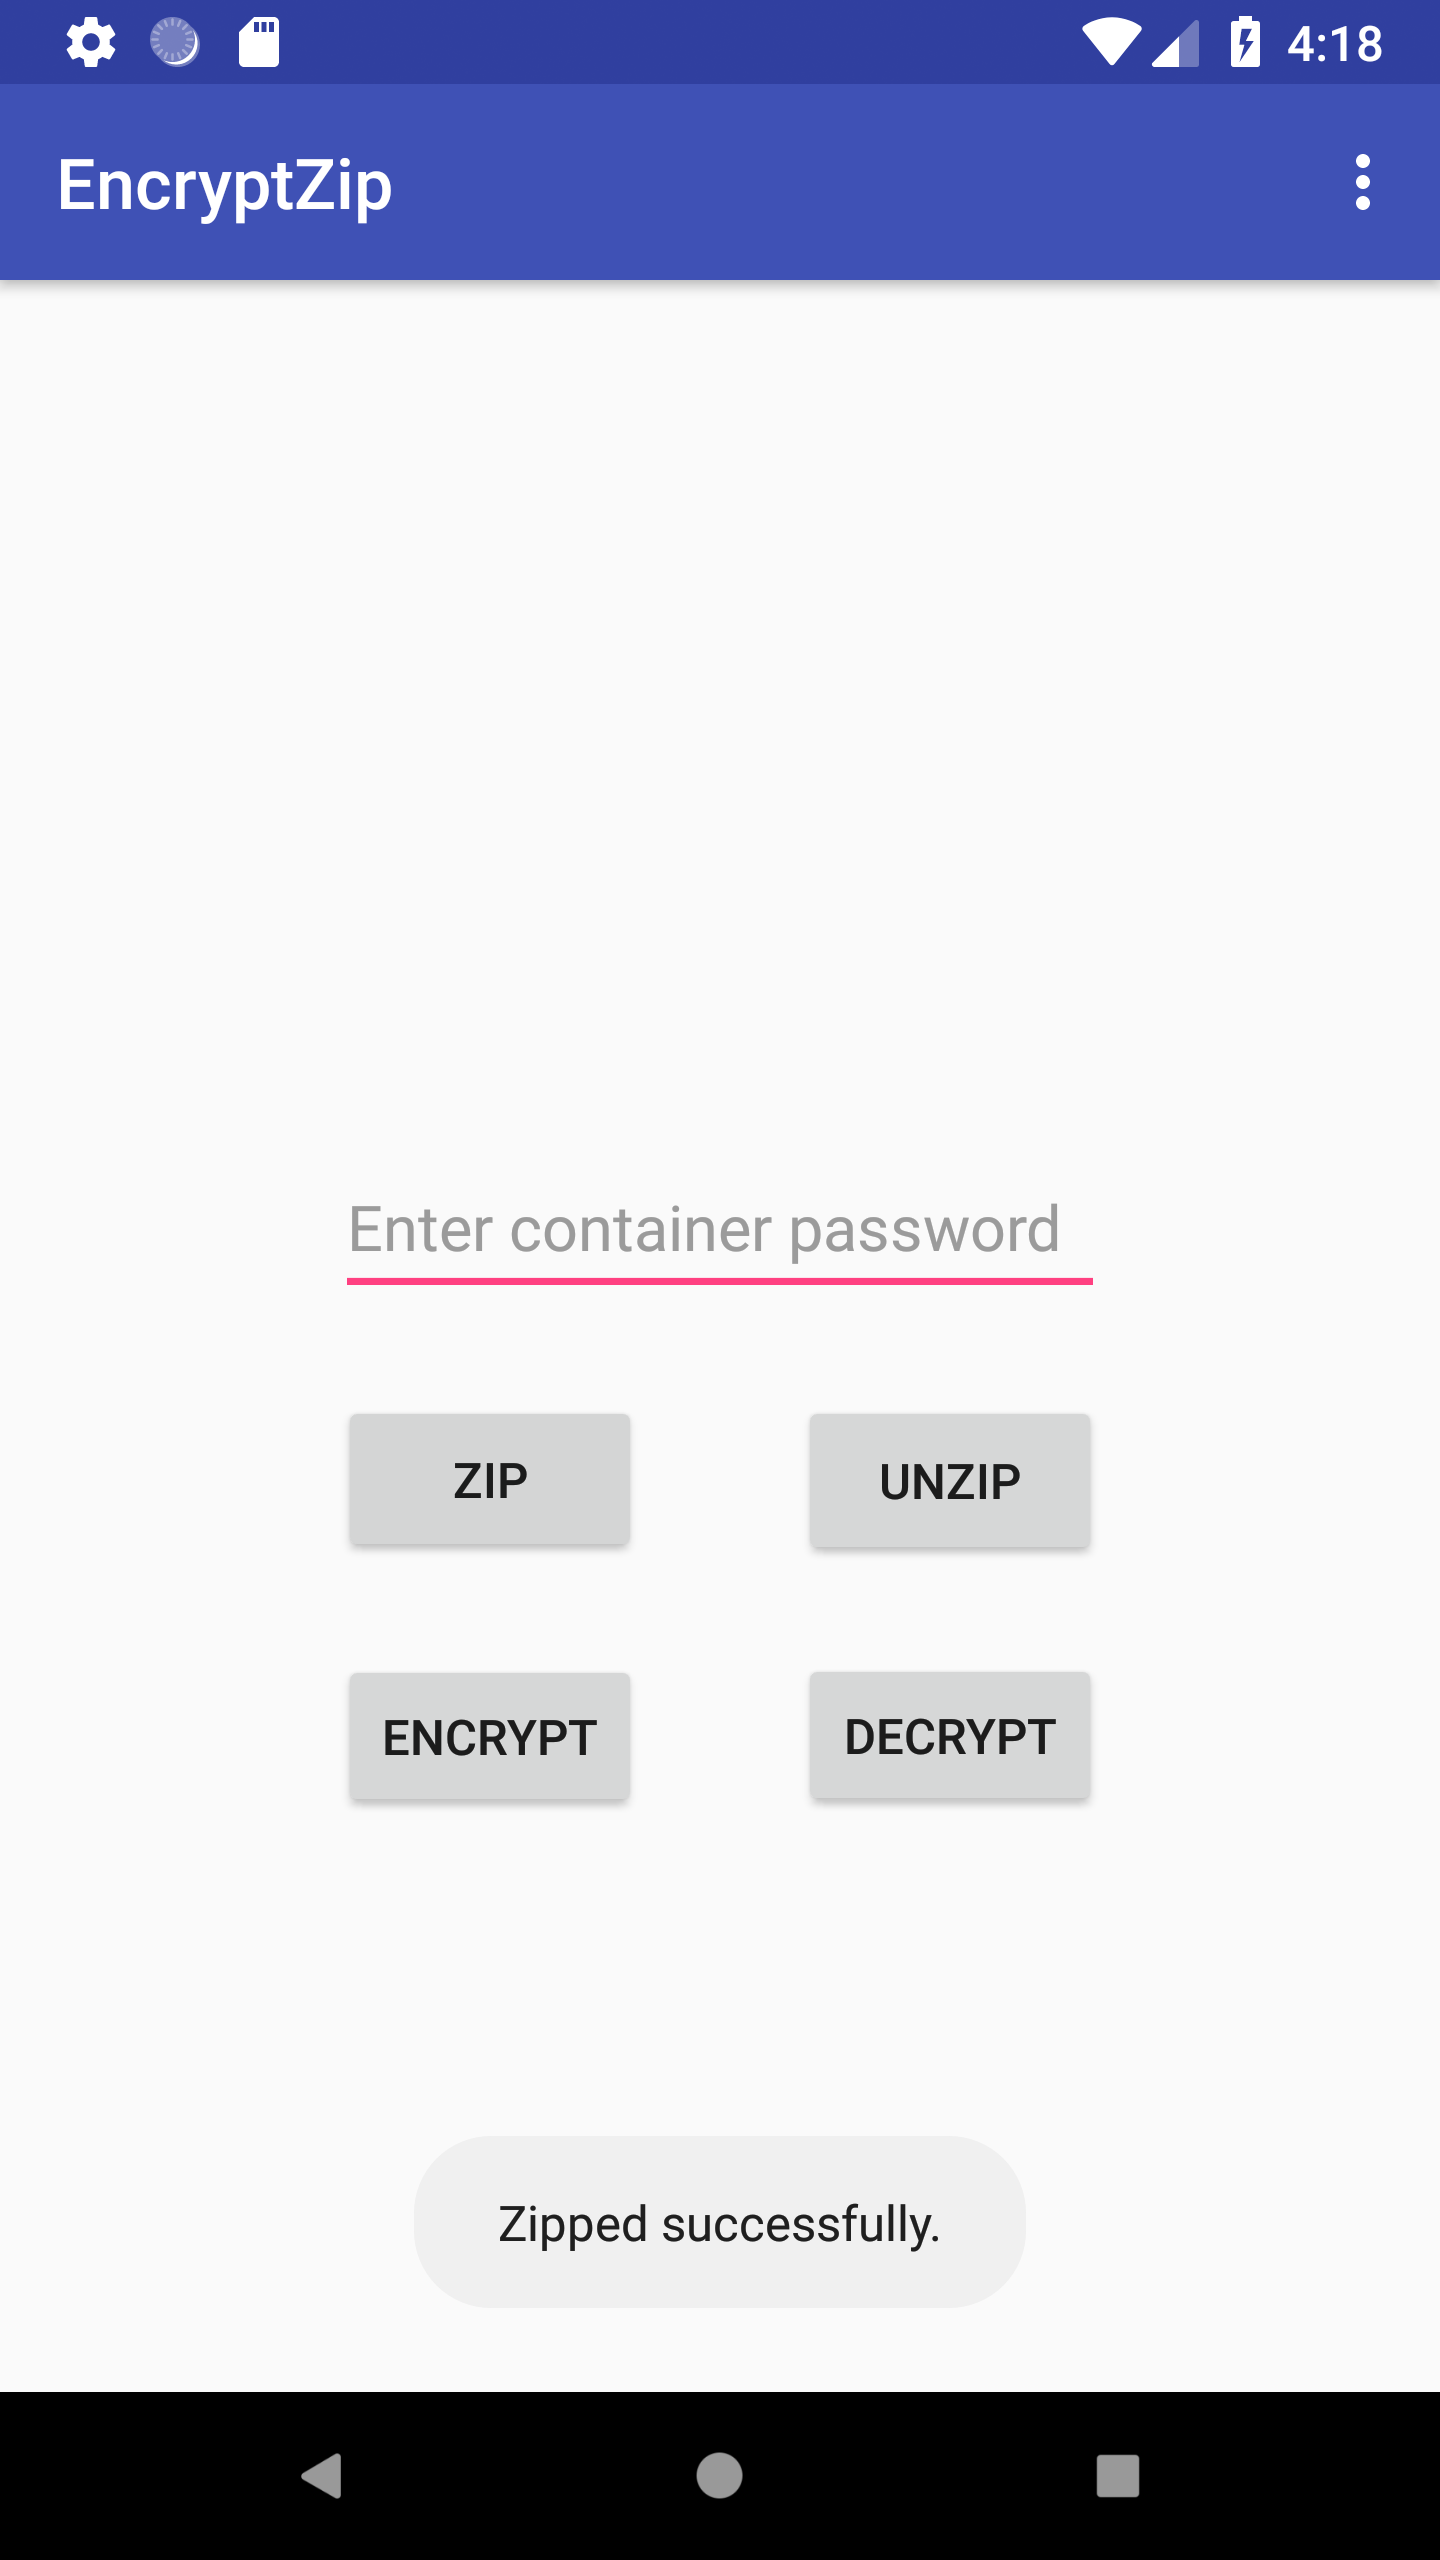
\includegraphics[width=4cm]{toast1}
\end{figure}
\begin{figure}[h]
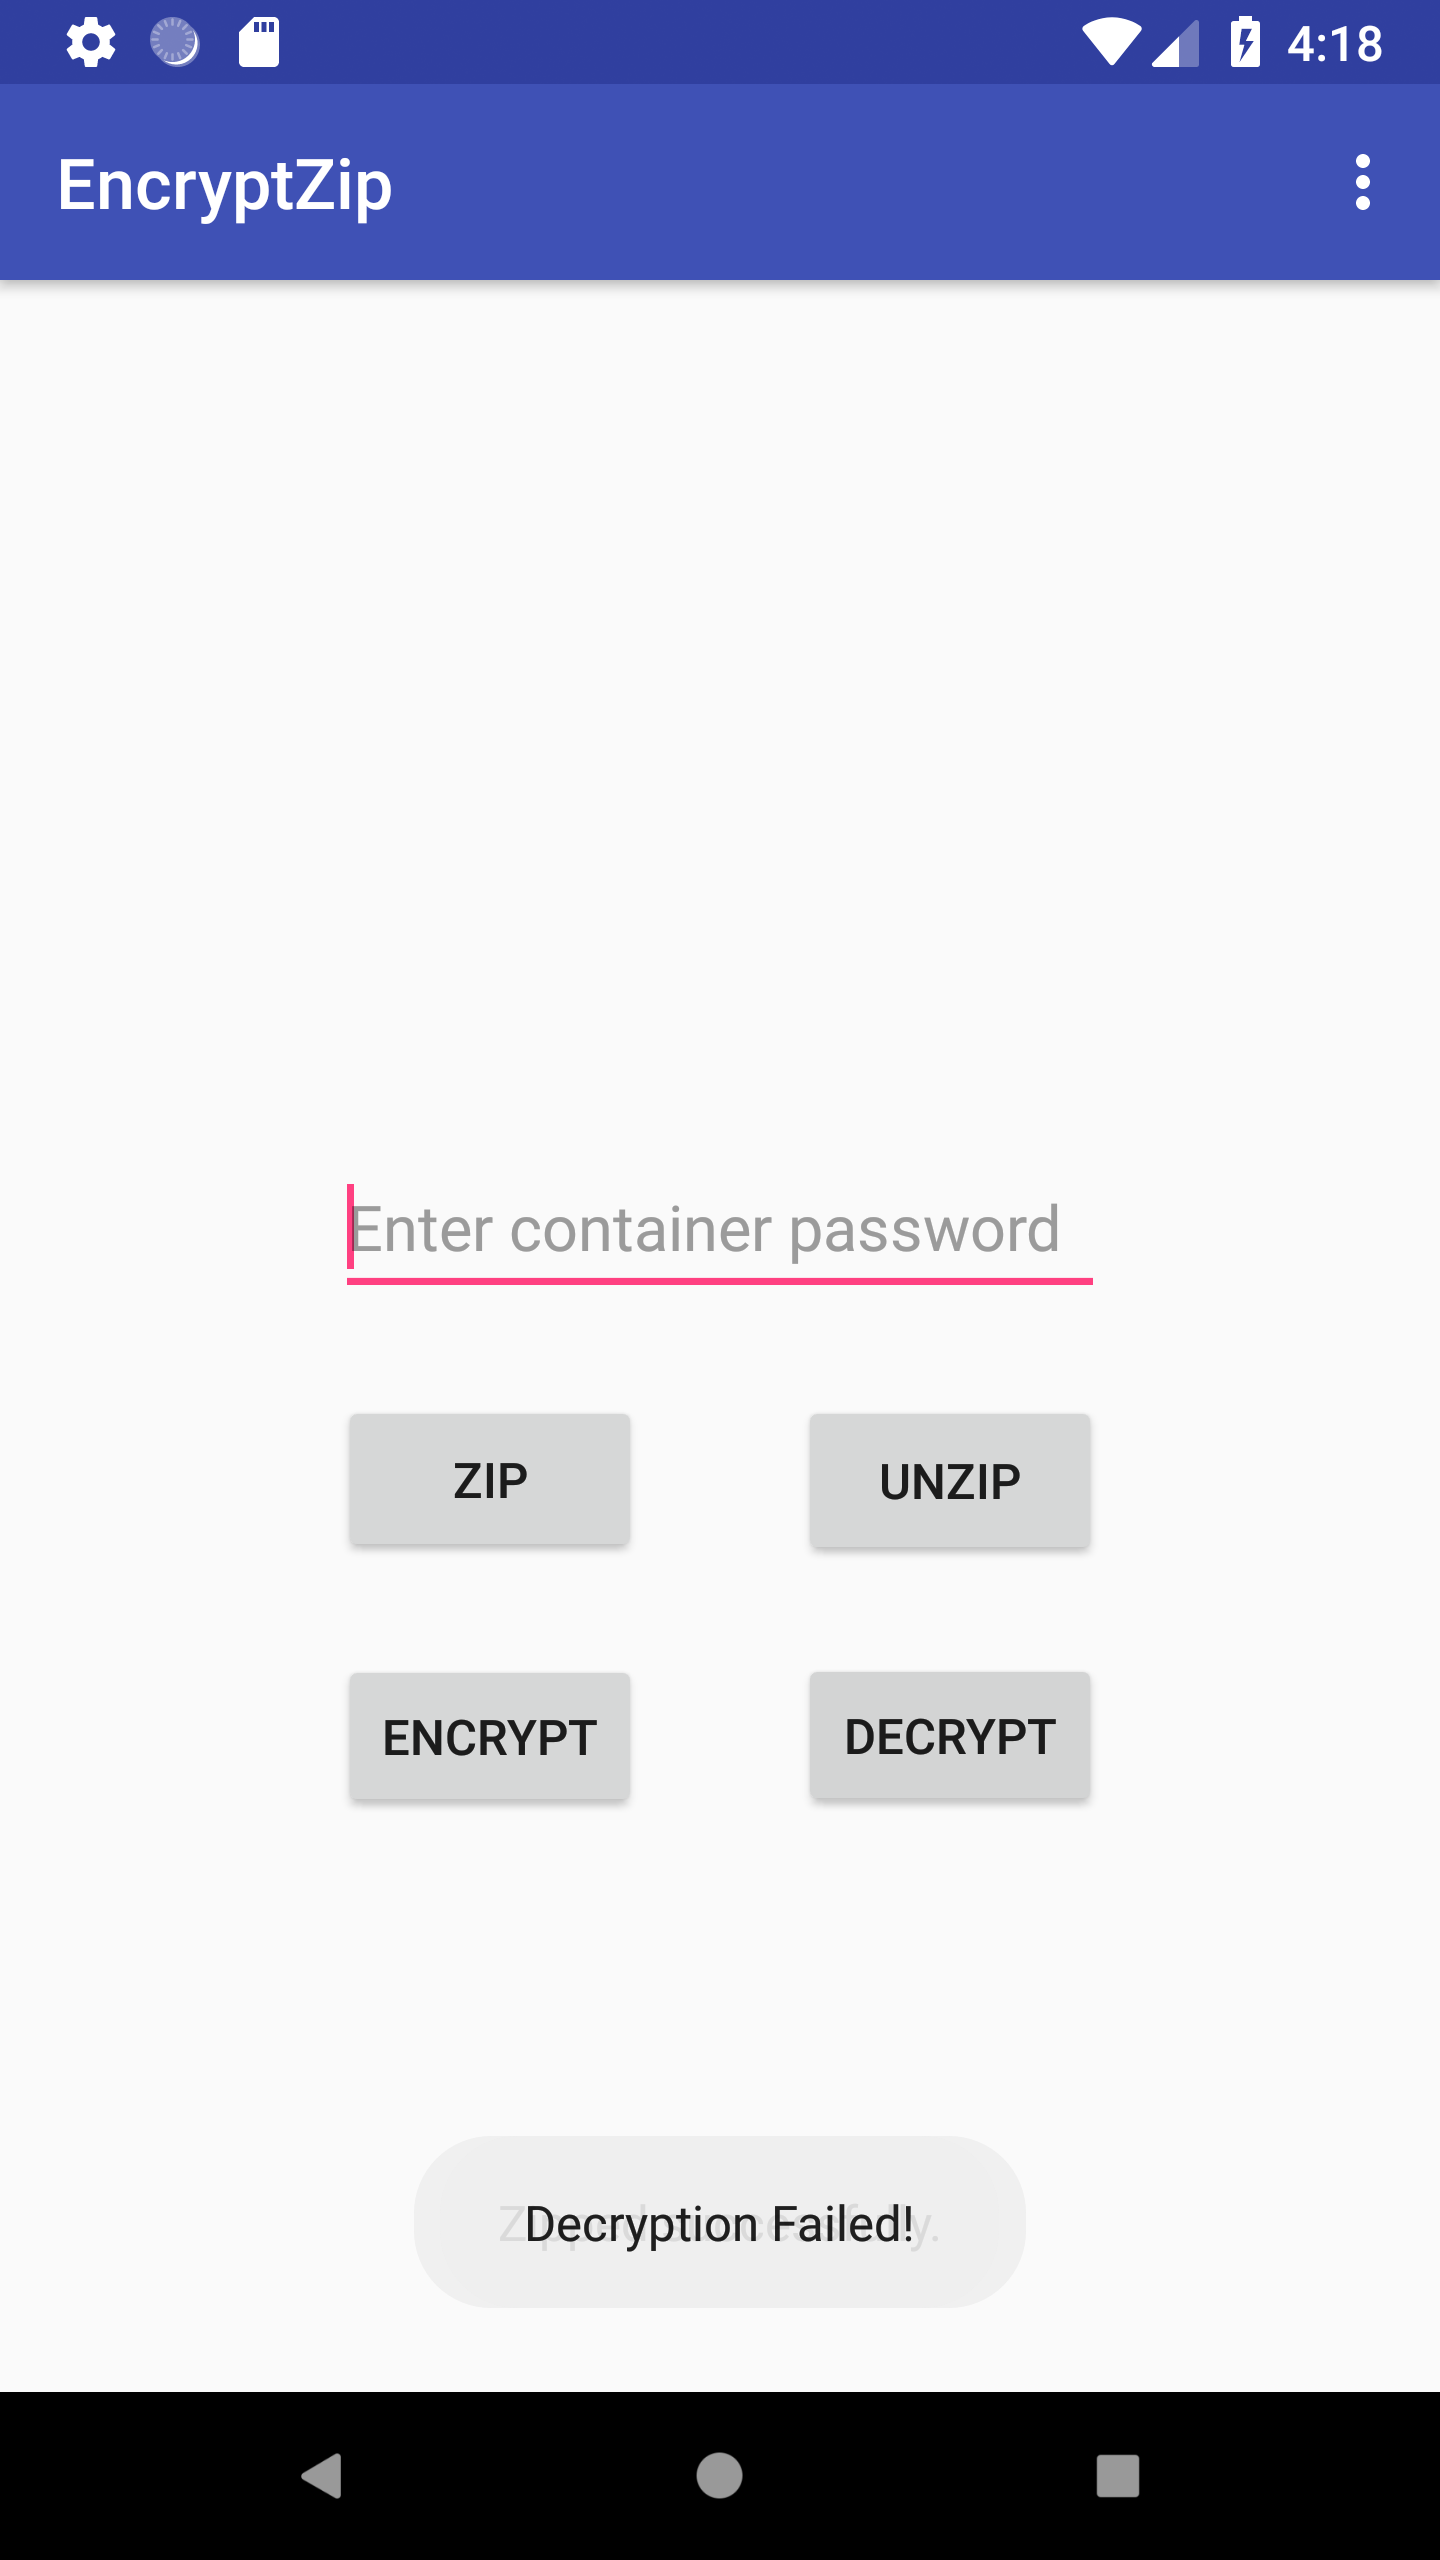
\includegraphics[width=4cm]{toast2}
\end{figure}

\clearpage

The data folder is accessible through the file system on Android devices. The contents of the data folder are zipped and the resulting zip file is stored in the zip folder.
\begin{figure}[H]
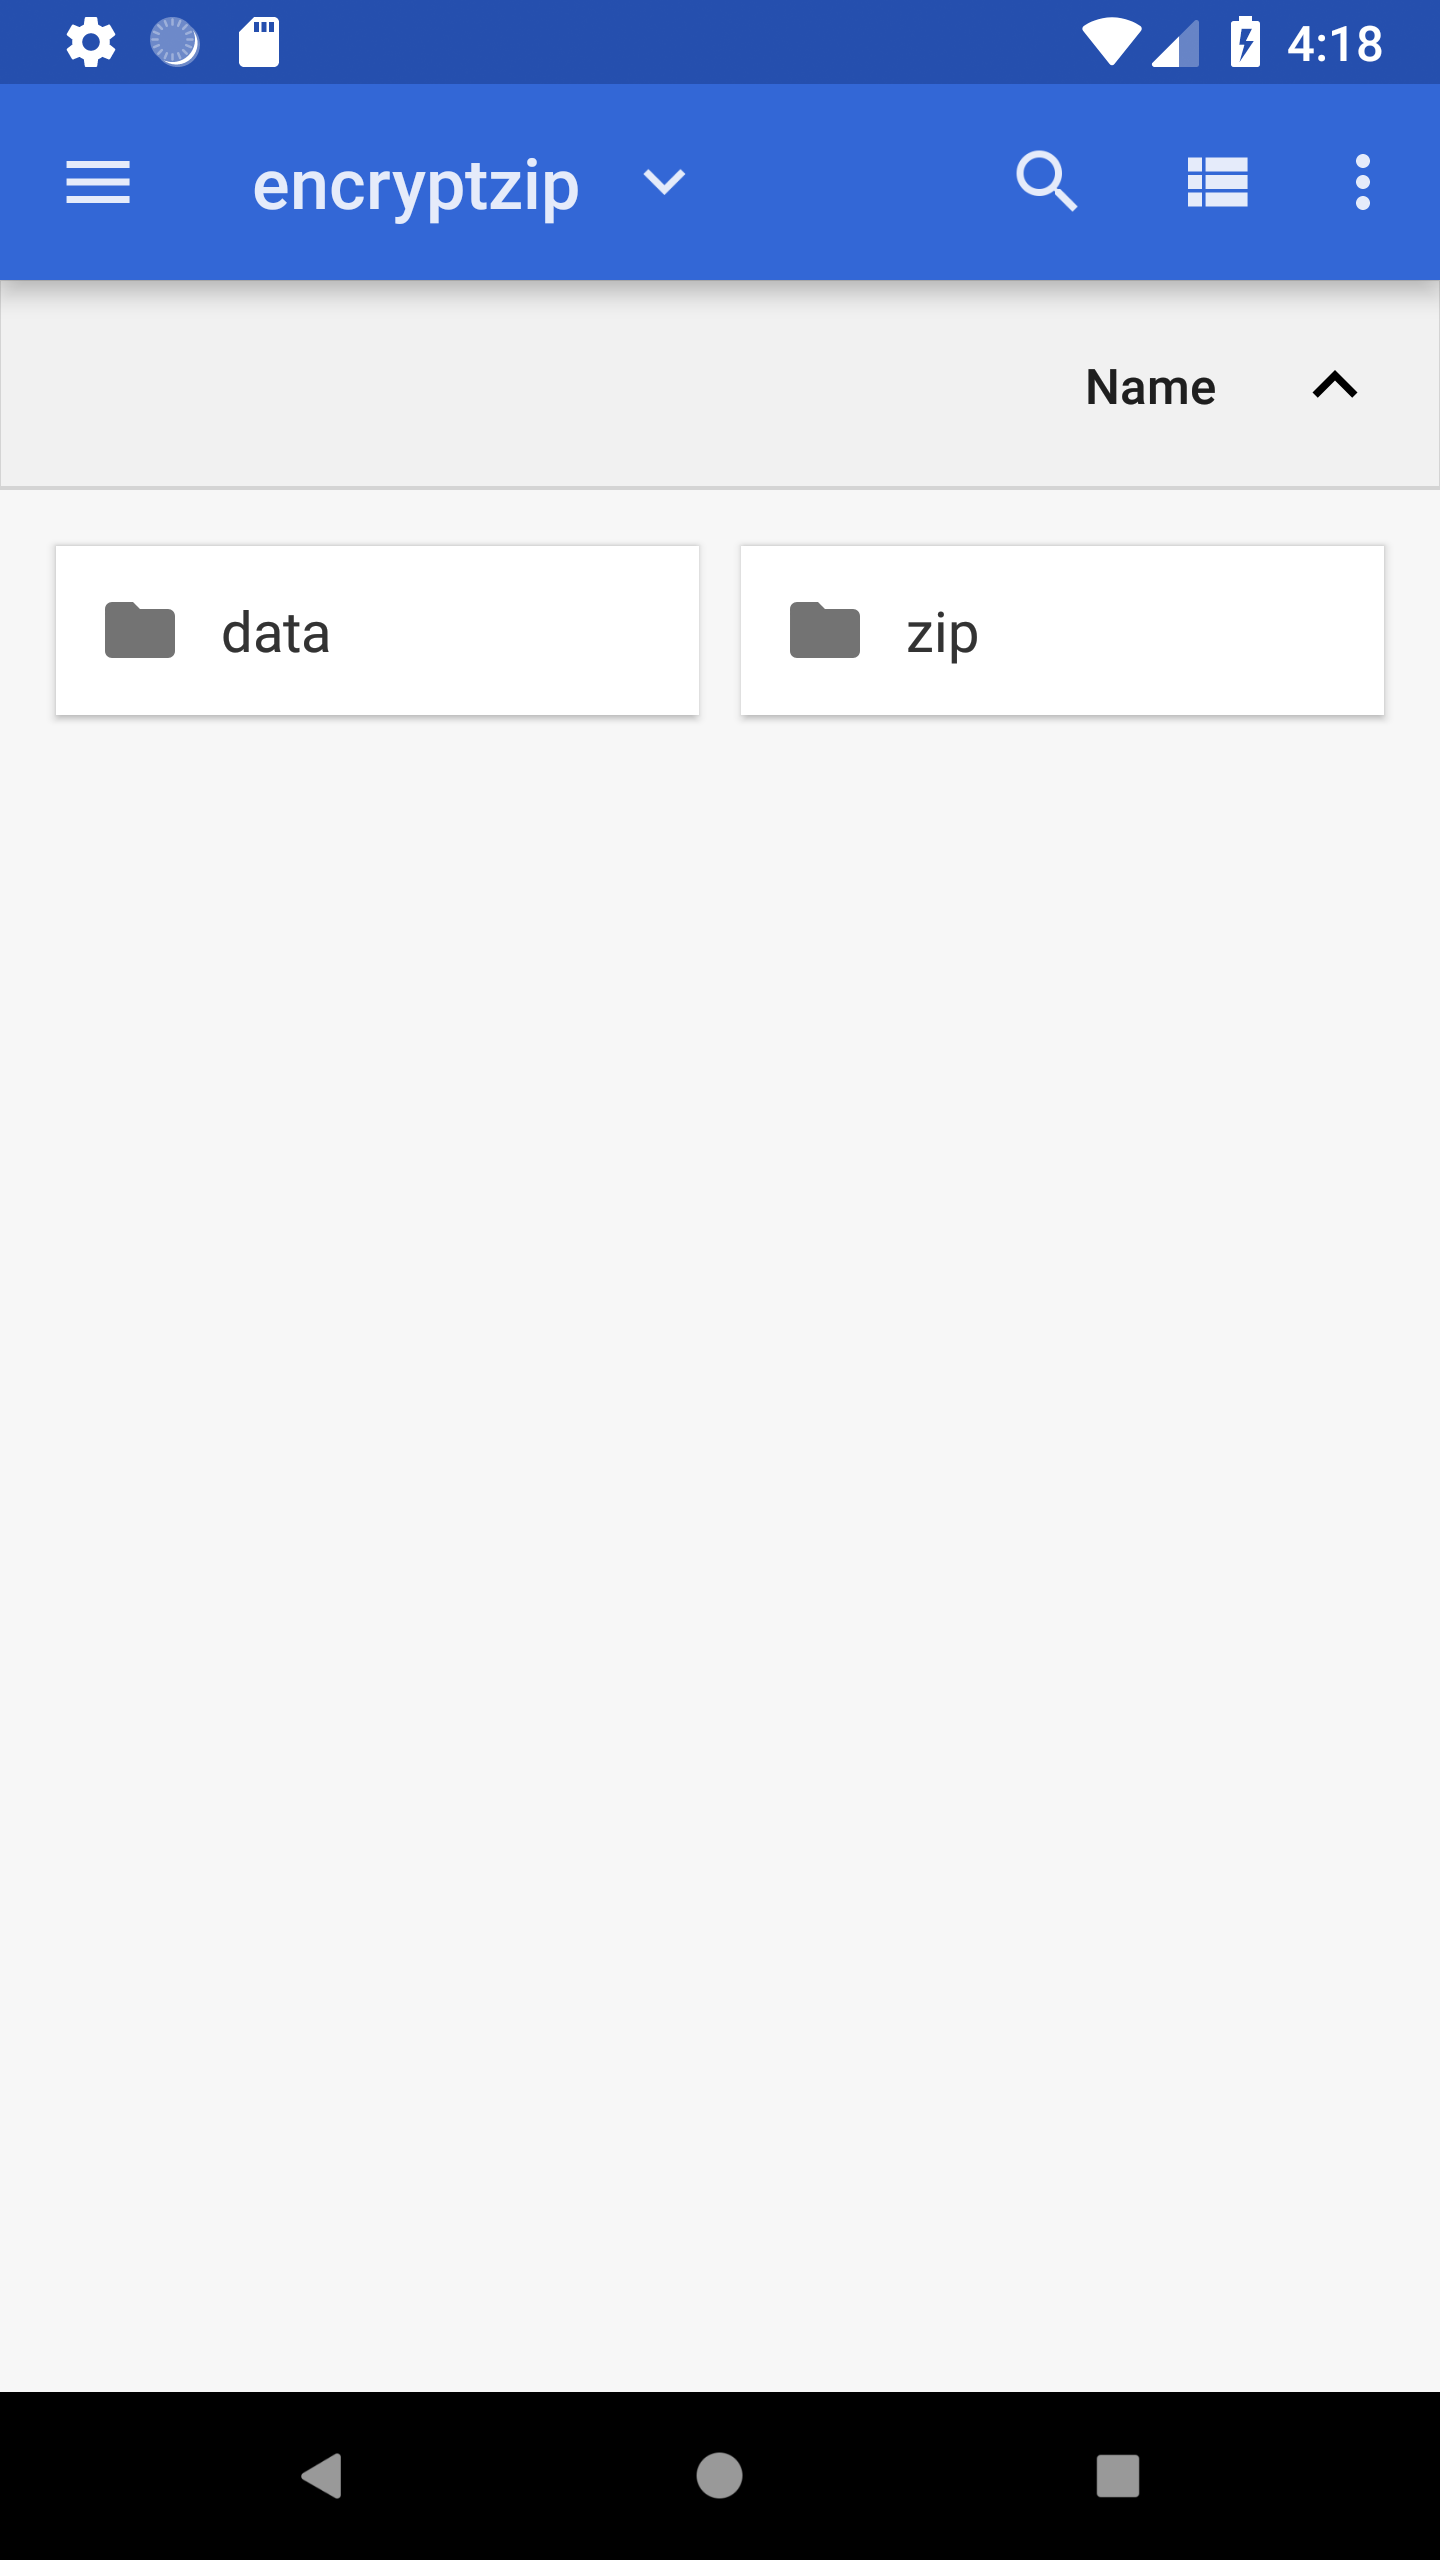
\includegraphics[width=8cm]{file1}
\end{figure}

\section{Conclusion}
stuff
\section{Sources}
stuff

\end{document}